\documentclass[notes,slidesec,a4]{seminar}
\usepackage[spanish]{babel}
\usepackage[utf8]{inputenc}

\usepackage{t-gsyc-6}
\usepackage{fancybox}
\usepackage{graphics}
\usepackage{moreverb}
\usepackage{alltt}
\usepackage{html}
\usepackage{hthtml}
\usepackage{amsmath}
\usepackage[normalsize]{subfigure}
\usepackage{url}
\usepackage{listings}

\usepackage{eurosym}

\title{Odometría visual con sensor RGBD en JdeRobot}
\author{Javier Benito Díaz}

\cop{Javier Benito Díaz}
\address{jbenito.dz@gmail.com}

\begin{document}
\maketitle

%%--------------------------------------------------------------

\begin{hslide}
	\slsect{Índice}
	\begin{itemize}
		\item Introducción 
		\item Objetivos
		\item Infraestructura
		\item Desarrollo
		\item Experimentos
		\item Conclusiones
	\end{itemize}
\end{hslide}

%%--------------------------------------------------------------

\begin{hslide}
	\slsect{Introducción}
	\slsubsect{Autolocalización visual}
	\begin{minipage}{6cm}
		\begin{center}
			\begin{figure}
				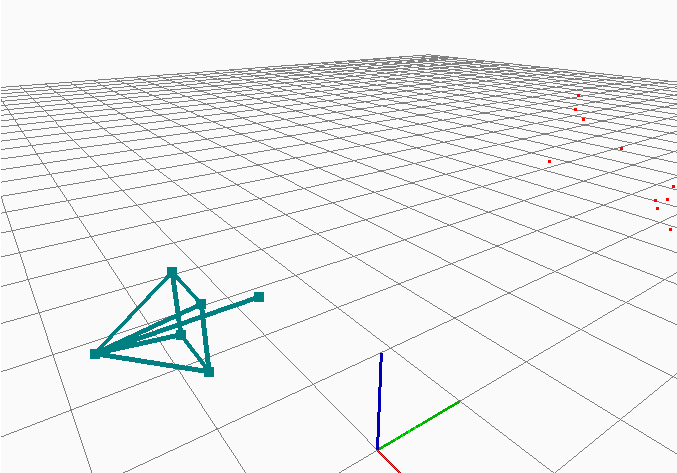
\includegraphics[width=6.0cm]{img/camera-opengl.png}
			\end{figure}
		\end{center}
	\end{minipage} \hfill
	\begin{minipage}{5cm}
		\begin{itemize}
			\item Estimar posición y orientación de la cámara.
			\item Información únicamente visual.
			\item Visión artificial.
		\end{itemize}
	\end{minipage}
\end{hslide}

%%--------------------------------------------------------------

\begin{hslide}
	\slsect{Introducción}
	\slsubsect{Autolocalización visual: aplicaciones}
	\begin{minipage}{5cm}
		\begin{itemize}
			\item Procesamiento de imágenes
			\item Medicina, OCR, Deportes, robótica...
			\item Realidad aumentada.
		\end{itemize}
	\end{minipage} \hfill
	\begin{minipage}{5cm}
		\begin{center}
			\begin{figure}
				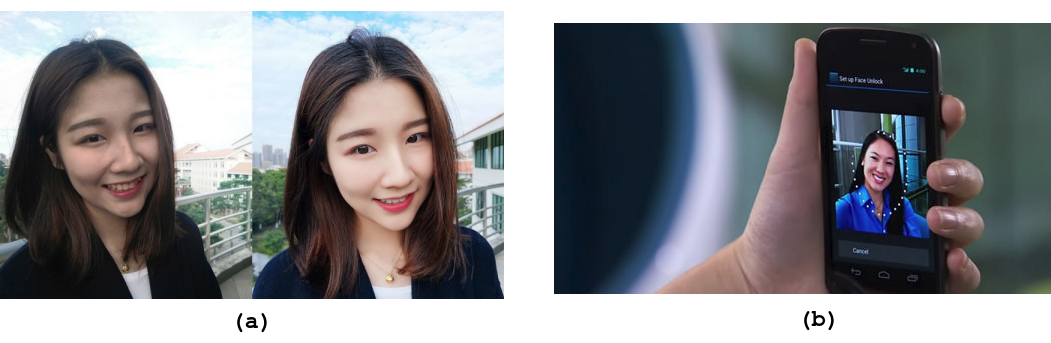
\includegraphics[width=6.0cm]{img/face.png}
				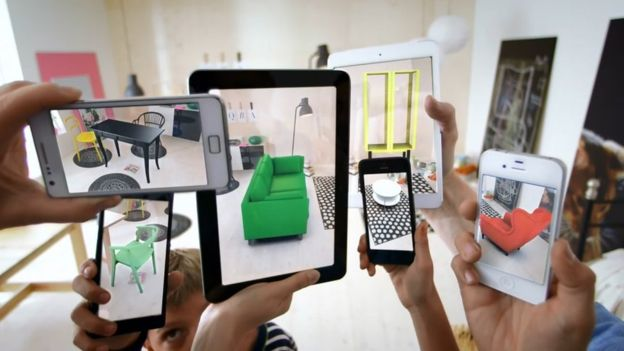
\includegraphics[width=3.0cm]{img/ikea.jpg}
			\end{figure}
		\end{center}

	\end{minipage}
\end{hslide}

%%--------------------------------------------------------------

\begin{hslide}
	\slsect{Introducción}
	\slsubsect{Autolocalización visual: Técnicas}
	\begin{minipage}{6cm}
		\begin{center}
			\begin{figure}
				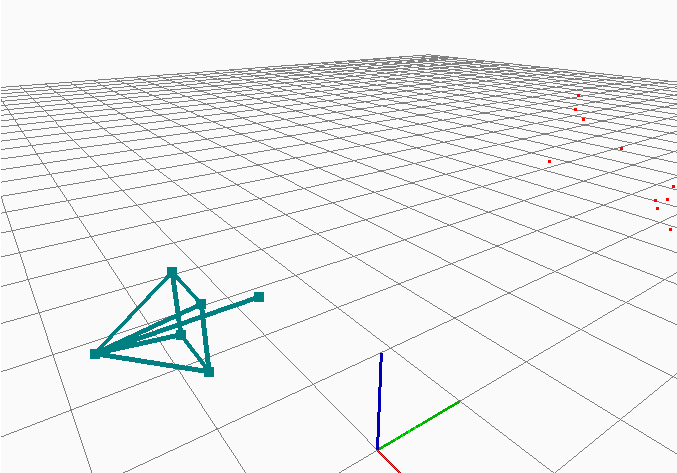
\includegraphics[width=6.0cm]{img/camera-opengl.png}
			\end{figure}
		\end{center}
	\end{minipage} \hfill
	\begin{minipage}{5cm}
		\begin{itemize}
			\item Structure from Motion (SfM).
			\item Visual SLAM.
			\begin{itemize}
				\item PTAM
			\end{itemize}
			\item Odometría visual.
		\end{itemize}
	\end{minipage}
\end{hslide}

%%--------------------------------------------------------------

\begin{hslide}
	\slsect{Objetivos}
			\begin{itemize}
			\item Desarrollar un programa que solucione el pro-
			blema de visualSLAM, para un sensor RGBD, a través de técnicas de odometría visual incrementales.
			\item Validación experimental del componente con datos obtenidos de un sensor real.
		\end{itemize}
		\begin{center}
			\begin{figure}
				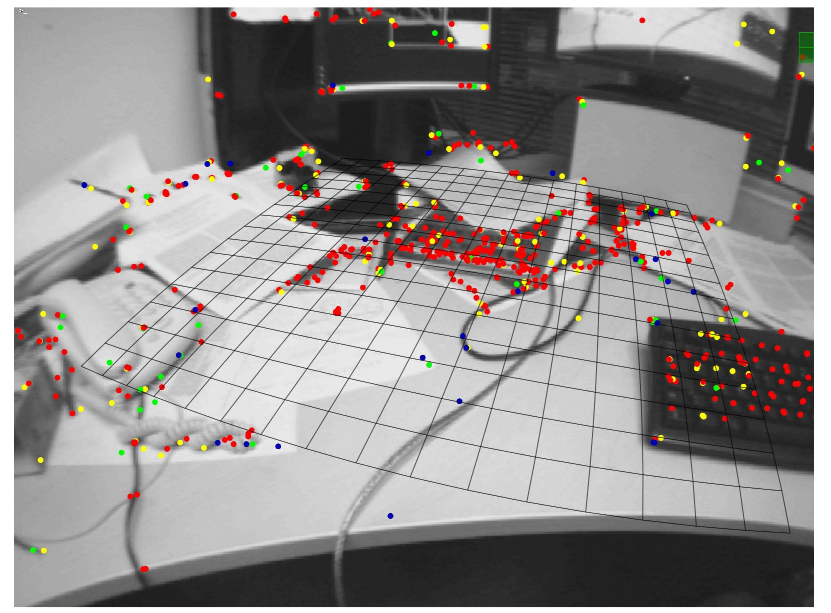
\includegraphics[width=5cm] {img/ptam.png}
			\end{figure}
		\end{center}
\end{hslide}

%--------------------------------------------------------------

\begin{hslide}
	\slsect{Infraestructura}
	\begin{minipage}{4cm}
		\begin{center}
			\begin{figure}
				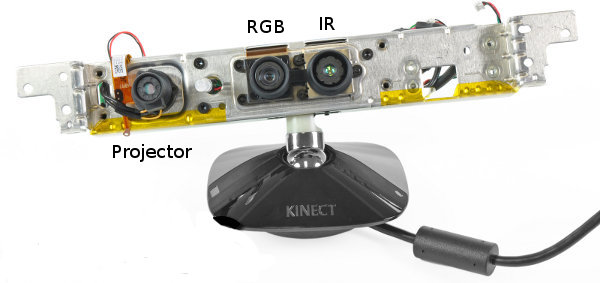
\includegraphics[width=5cm] {img/ros_kinect.jpg}
				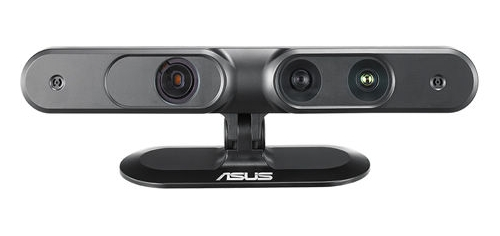
\includegraphics[width=5cm] {img/xtion-pro-live.jpg}
			\end{figure}
		\end{center}
	\end{minipage} \hfill
	\begin{minipage}{5cm}
		\begin{itemize}
			\item Sensores RGBD
			\item JdeRobot 5.4.0
			\begin{itemize}
				\item Biblioteca Progeo
				\item Servidor OpenniServer
			\end{itemize}
			\item ICE de comunicaciones
			\item Point Cloud Library (PCL)
			\item OpenCV
			\item Eigen
			\item Interfaz gráfica GTK+
			\item OpenGL
		\end{itemize}
	\end{minipage}
\end{hslide}

\end{document}